\begin{enunciado}{\ejercicio}
  Sean $A$ y $B \en K^{n \times n}$. Probar que:
  \begin{enumerate}[label=(\alph*)]
    \item Si $A \ytext B$ son triangulares superiores, $AB$ es triangular superior.
    \item Si $A \ytext B$ son diagonales, $AB$ es diagonal.
    \item Si $A$ es estrictamente triangular superior (es decir, $a_{ij} = 0$ si $i\geq j$), $A^n = 0$.
  \end{enumerate}
\end{enunciado}

\def\triangularSuperior{
  \begin{tikzpicture}[baseline=-6, scale = 0.5]
    \draw[blue, thin, fill=blue!20,yshift = -4, xshift = -8] (-1,1) -- (1.7,1) -- (1.7,-0.7) -- cycle;
    \node at (0,0) {
      $
        \matriz{cc}{
          \quad &  a_{\green{i}\blue{j}} \\
          0 &
        }
      $
    };
  \end{tikzpicture}
}

\def\diagonal{
  \begin{tikzpicture}[baseline=-6, scale = 0.5]
    \draw[blue, thin, fill=blue!20,yshift = 0, xshift = 0, rotate = -45] (-1.1,0.3) rectangle (1.1,-.3);
    \node at (0,0) {
      $
        \matriz{cc}{
          &  0 \\
          0 &
        }
      $
    };
  \end{tikzpicture}
}

\def\triangularSuperiorEstricta{
  \begin{tikzpicture}[baseline=-6, scale = 0.5]
    \draw[blue, thin, fill=blue!20,yshift = 0, xshift = 0] (-0.6,0.8) -- ++(0,-0.5) -- (0.2,-0.1) -- ++(0.8,0) -- (1,0.8) -- cycle;
    \node at (0,0) {
      $
        \matriz{cc}{
          0 &  a_{\green{i}\blue{j}} \\
          0 & 0
        }
      $
    };
  \end{tikzpicture}
}

\begin{enumerate}[label=(\alph*)]
  \item  Una matriz $A$ va a ser triangular superior si todos los número debajo de la diagonal son cero:
        $$
          A_{\green{i}\blue{j}}
          \igual{$\llamada1$}
          \llave{ccl}{
            0 & \text{ si } & \green{i} > \blue{j} \\
            a_{\green{i}\blue{j}} & \text{ si } & \green{i} \leq \blue{j}
          }
          \qquad
          \triangularSuperior
        $$
        Los $a_{\green{i}\blue{j}}$ no tienen que  ser necesariamente distinto a cero. Ahora multiplico dos matrices triangulares superiores:
        $$
          [A \cdot B]_{\green{i}\blue{j}} = \sumatoria{\purple{k} = 1}{n} a_{\green{i}\purple{k}} \cdot b_{\purple{k}\blue{j}}
          =
          a_{\green{i}\purple{1}} \cdot b_{\purple{1}\blue{j}} + a_{\green{i}\purple{2}} \cdot b_{\purple{2}\blue{j}} + \cdots + a_{\green{i}\purple{n}} \cdot b_{\purple{n}\blue{j}}
          \igual{$\llamada1$}
          \llave{cc}{
            \sumatoria{\green{i} \leq \purple{k}\leq  \blue{j}}{} a_{\green{i}\purple{k}} \cdot b_{\purple{k}\blue{j}} & \llamada2 \\
            0 & \text{ en otro caso}
          }
        $$
        Se cumple $\llamada2$ son los que tiene las
        \textit{\green{filas} menores o iguales \purple{columnas}} y \textit{\purple{filas} menores o iguales \blue{columnas}},
        si no son cero. Básicamente la definición de matriz triangular superior.

  \item Esta es un poco más fácil. Una matriz es diagonal si:
        $$
          A_{ij}
          \igual{$\llamada1$}
          \llave{ccl}{
            0 & \text{ si } & i \distinto j\\
            a_{ij} &\text{ si } & i = j
          }
          \qquad \diagonal
        $$
        Nuevamente, los elementos diagnonales no tienen que ser necesariamente distintos de cero. Ahora multiplico dos matrices diagonales:
        $$
          [A \cdot B]_{\green{i}\blue{j}} = \sumatoria{\purple{k} = 1}{n} a_{\green{i}\purple{k}} \cdot b_{\purple{k}\blue{j}}
          =
          a_{\green{i}\purple{1}} \cdot b_{\purple{1}\blue{j}} + a_{\green{i}\purple{2}} \cdot b_{\purple{2}\blue{j}} + \cdots + a_{\green{i}\purple{n}} \cdot b_{\purple{n}\blue{j}}
          \igual{$\llamada1$}
          \llave{cc}{
            a_{\green{i}\purple{i}}\cdot b_{\purple{i}\blue{i}} & \llamada2\\
            0 & \text{ en otro caso }
          }
        $$
        En la sumatoria las \purple{columnas} de los elementos de $A$ coinciden con las filas de los elementos de $B$, pero
        solo cuando estemos multiplicando la \green{fila} $i$ con la \blue{columna} $i$ es que ambos elementos podrían ser no nulos.

  \item  Una matriz $A$ va a ser triangular superior estricta si todos los número debajo y de la diagonal son cero:
        $$
          A_{\green{i}\blue{j}}
          \igual{$\llamada1$}
          \llave{ccl}{
            0 & \text{ si } & \green{i} \geq \blue{j} \\
            a_{\green{i}\blue{j}} & \text{ si } & \green{i} < \blue{j}
          }
          \qquad \triangularSuperiorEstricta
        $$
        Meto inducción porque es un viaje.
        Quiero probar que:
        $$
          p(n) : A \en K^{n \times n} \text{ estrictamente triangular superior} \entonces A^n = 0.
        $$
        \textit{Caso base:}
        $$
          p(\blue{2}) : A \en K^{\blue{2} \times \blue{2}} \text{ estrictamente triangular superior} \entonces A^{\blue{2}} = 0
        $$
        Cálculo directo
        $$
          A \cdot A\matriz{cc}{
            0 & a_{12} \\
            0 & 0
          }
          \cdot
          \matriz{cc}{
            0 & a_{12} \\
            0 & 0
          }
          =
          \matriz{cc}{
            0 & 0 \\
            0 & 0
          }
        $$
        por lo tanto $p(\blue{2})$ es verdadera.

        \medskip

        \textit{Paso inductivo:}
        Voy a asumir que para algún $\blue{k} \en \enteros$
        $$
          p(\blue{k}) : \ub{A \en K^{\blue{k} \times \blue{k}} \text{ estrictamente triangular superior} \entonces A^{\blue{k}} = 0}{\text{\purple{hipótesis inductiva}}}
        $$
        es verdadera. Por lo tanto ahora quiero probar que:
        $$
          p(\blue{k+1}) : A \en K^{(\blue{k+1}) \times (\blue{k+1})} \text{ estrictamente triangular superior} \entonces A^{\blue{k+1}} = 0
        $$
        Para probar esta tremenda garompa, voy a usar el producto en bloques.
        Tengo una matriz $A \en K^{(\blue{k+1}) \times (\blue{k+1})}$ estrictamente triangular superior y la parto en bloques así:
        $$
          \begin{tikzpicture}[baseline=0, scale = 1]
            \draw[blue, thin, fill=blue!10,yshift = 0, xshift = 0] (-37px, 20px) rectangle ++(13px,13px);
            \draw[OliveGreen, thin, fill=OliveGreen!10,yshift = 0, xshift = 0] (-20px, 20px) rectangle ++(80px,13px);
            \draw[orange, thin, fill=orange!10,yshift = 0, xshift = 0] (-20px, -32px) rectangle ++(80px,50px);
            \draw[violet, thin, fill=violet!10,yshift = 0, xshift = 0] (-37px, -32px) rectangle ++(13px,50px);
            \node at (0,0) {
              $
                A =
                \matriz{c|ccc}{
                  \yellow{0} & \violet{a_{12}} & \violet{\cdots} & \violet{a_{1 \blue{k+1}}} \\ \hline
                  \red{0} & \green{0} & \green{\ddots} & \green{\vdots} \\
                  \red{\vdots} & \green{0} & \green{\ddots} & \green{a_{k \blue{k+1}}} \\
                  \red{0} & \green{0} & \green{0} & \green{0}
                }
              $
            };
          \end{tikzpicture}
        $$
        \def\bloques{
          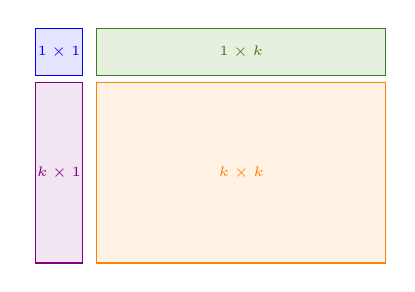
\begin{tikzpicture}[baseline=0, scale = 1.3, every node/.style={font=\tiny}]
            \draw[blue, thin, fill=blue!10,yshift = 0, xshift = -12] (-37px, 20px) rectangle ++(13px,13px) node[midway]{$1\times 1$};
            \draw[OliveGreen, thin, fill=OliveGreen!10,yshift = 0, xshift = -12] (-20px, 20px) rectangle ++(80px,13px) node[midway]{$1\times k$};
            \draw[orange, thin, fill=orange!10,yshift = 0, xshift = -12] (-20px, -32px) rectangle ++(80px,50px) node[midway]{$k \times k$};
            \draw[violet, thin, fill=violet!10,yshift = 0, xshift = -12] (-37px, -32px) rectangle ++(13px,50px)node[midway]{$k \times 1$};
          \end{tikzpicture}
        }
        \def\bloqueAzul{
          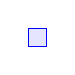
\begin{tikzpicture}[baseline=10, scale = 0.5, every node/.style={font=\tiny}]
            \draw[blue, thin, fill=blue!10,yshift = 0, xshift = -12] (-37px, 20px) rectangle ++(13px,13px);
          \end{tikzpicture}
        }
        \def\bloqueAzulZ{
          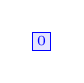
\begin{tikzpicture}[baseline=10, scale = 0.5, every node/.style={font=\tiny}]
            \draw[blue, thin, fill=blue!10,yshift = 0, xshift = -12] (-37px, 20px) rectangle ++(13px,13px) node[midway]{$0$};
          \end{tikzpicture}
        }
        \def\bloqueVioletZ{
          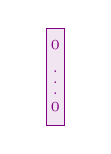
\begin{tikzpicture}[baseline=0, scale = 0.5, every node/.style={font=\tiny}]
            \draw[violet, thin, fill=violet!10,yshift = 0, xshift = -12] (-37px, -32px) rectangle ++(13px,70px)
            node[midway]{$
                  \begin{array}{c}
                    0      \\
                    \vdots \\
                    0
                  \end{array}
                $
              };
          \end{tikzpicture}
        }
        \def\bloqueViolet{
          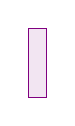
\begin{tikzpicture}[baseline=0, scale = 0.5, every node/.style={font=\tiny}]
            \draw[violet, thin, fill=violet!10,yshift = 0, xshift = -12] (-37px, -32px) rectangle ++(13px,50px);
          \end{tikzpicture}
        }
        \def\bloqueVerde{
          
\begin{tikzpicture}[baseline=0, scale = 0.5, every node/.style={font=\tiny}]
            \draw[OliveGreen, thin, fill=OliveGreen!10, yshift = -20, xshift = -12] (-50px, 20px) rectangle ++(80px,13px);
          \end{tikzpicture}
        }
        \def\bloqueVerdeZ{
          
\begin{tikzpicture}[baseline=0, scale = 0.5, every node/.style={font=\tiny}]
            \draw[OliveGreen, thin, fill=OliveGreen!10, yshift = -20, xshift = -12] (-20px, 20px) rectangle ++(160px,13px) node[midway]{$0 \cdots\cdots\cdots 0$};
          \end{tikzpicture}
        }
        \def\bloqueOrange{
          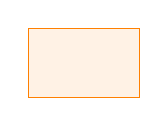
\begin{tikzpicture}[baseline=0, scale = 0.5, every node/.style={font=\tiny}]
            \draw[orange, thin, fill=orange!10,yshift = 0, xshift = -12] (-20px, -32px) rectangle ++(80px,50px);
          \end{tikzpicture}
        }
        \def\bloqueOrangeZ{
          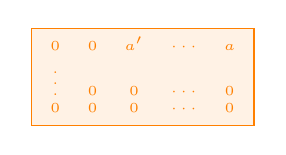
\begin{tikzpicture}[baseline=0, scale = 0.5, every node/.style={font=\tiny}]
            \draw[orange, thin, fill=orange!10,yshift = 0, xshift = -12] (-20px, -32px) rectangle ++(160px,70px)
            node[midway]{
                $
                  \begin{array}{ccccc}
                    0      & 0 & a' & \cdots & a \\
                    \vdots & 0 & 0  & \cdots & 0 \\
                    0      & 0 & 0  & \cdots & 0 \\
                  \end{array}
                $};
          \end{tikzpicture}
        }
        $$
          \begin{array}{rcl}
            A^2 = A \cdot A                                            & =                                                          & \bloques \times \bloques \\ \\
                                                                       & =                                                          &
            \matriz{c|c}{
            \bloqueAzul\ \bloqueAzul + \bloqueVerde\ \bloqueViolet     & \bloqueAzul\ \bloqueVerde + \bloqueVerde\ \bloqueOrange                               \\ \hline
            \bloqueViolet\ \bloqueAzul +  \bloqueOrange\ \bloqueViolet & \bloqueViolet\ \bloqueVerde + \bloqueOrange\ \bloqueOrange
            }                                                                                                                                                  \\
                                                                       & =                                                          &
            \matriz{c|c}{
            \bloqueAzulZ                                               & \bloqueVerdeZ                                                                         \\ \hline
            \bloqueVioletZ                                             & \bloqueOrangeZ
            }
          \end{array}
        $$
        Oka, esto se fue al carajo.
        Pero está demostrado.
        La última matriz, es el resultado de $A^2$. Tiene todos ceros excepto en el \orange{bloque naranja}, que está en $K^{\blue{k} \times \blue{k}}$ y es
        el producto de hacer el \orange{bloque naranja} por el \orange{bloque naranja} dado que el \violet{bloque violeta} por el \green{bloque verde} dio 0.
        Por lo tanto el \orange{bloque naranja} es la \purple{hipótesis inductiva}\red{!!!} Multiplicar $k+1$ veces $A$ por si misma dará 0, porque el producto,
        será el (\orange{bloque naranja})$^2$ con cada vez más ceros.
\end{enumerate}

Dado que $p(2), p(k) \ytext p(k+1)$ resultaron verdaderas, por el principio de inducción en $p(n)$ también será verdadera  $\paratodo n \en \naturales$

El caso con $n=1$ es trivial, dejame en paz.

\begin{aportes}
  \item \aporte{\dirRepo}{naD GarRaz \github}
\end{aportes}
